\documentclass{discussion}

\usepackage{amsmath, amsthm, amssymb}
% \usepackage{xcolor, hyperref, cleveref}
\usepackage{mathtools}
\usepackage{derivative}
\usepackage{tabularx}
\usepackage{graphicx}
\usepackage{tasks}
\usepackage{mdframed}
\usepackage{commands}

\settasks{
    label-width = 13.99168pt,
    item-indent = 17.6413pt,
}

\discussion{3}
\author{Sections B04 and B06}
\date{Fall 2024}

\begin{document}

\section{More convergence tests}

\begin{question}
    Determine whether the following series converge or diverge.
    State which test you used.
    \begin{tasks}[label={\arabic*.}](2)
        % Divergence test
        \task \(\displaystyle \sum_{n=1}^\infty (-1)^n \cdot 2^{1/n}\)
        % Comparison with geometric series, convergent
        \task \(\displaystyle \sum_{n=1}^\infty \frac{5 \cdot 2^{n+1}}{3^{n-1}}\)
        % Absolute convergence test, comparison with geometric series or root test, convergent
        \task \(\displaystyle \sum_{n=1}^\infty \cos(n) 2^{-(n^2)}\)
        % alternating series, convergent
        \task \(\displaystyle \sum_{n=1}^\infty \frac{\cos(\pi n)}{\sqrt{n}}\)
        % ratio test, convergent
        \task \(\displaystyle \sum_{n=1}^\infty \frac{n!}{\sqrt{(2n)!}}\)
        % Divergent test, ratio test
        \task \(\displaystyle \sum_{n=1}^\infty \left( \frac{5}{4} \right)^n \left( \frac{4n}{5n + 1} \right)\)
        % Comparison with p-series, convergent
        \task \(\displaystyle \sum_{n=1}^\infty \sin^2\left( \frac{1}{n} \right)\)
        % root test, convergent
        \task \(\displaystyle \sum_{n=1}^\infty \sin^n\left( 1 + \frac{1}{n} \right)\)
        % root test, convergent
        \task \(\displaystyle \sum_{n=1}^\infty \left( 1 - \frac{1}{n} \right)^{(n^2)}\)
        % root test, ratio test, convergent, comparison with p series
        \task \(\displaystyle \sum_{n=1}^\infty \frac{n!}{n^n}\)
    \end{tasks}
\end{question}

\vspace{1em}

\begin{question}
    The following boxed argument \textbf{falsely concludes} that the series \(\displaystyle \sum_{n=1}^\infty \frac{1 + 2(-1)^n}{n}\) converges.
    Identify the mistake(s) and provide a correct argument for the divergence of the series.
    \begin{mdframed}
        Notice that
        \begin{equation*}
            \sum_{n=1}^\infty \frac{1 + 2(-1)^n}{n} = -\frac{1}{1} + \frac{3}{2} - \frac{1}{3} + \frac{3}{4} - \frac{1}{5} + \frac{3}{6} - \dots
        \end{equation*}
        is an alternating series and the limit of \(-\frac{1}{n} \leq \frac{1 + 2(-1)^n}{n} \leq \frac{3}{n}\) as \(n \to \infty\) is \(0\) by the sandwich theorem.
        Thus, it converges by the alternating series test.
    \end{mdframed}
\end{question}

\vspace{1em}

\begin{question}[More practice]
    Determine whether the following series converge or diverge.
    State which test you used.
    \begin{tasks}[label={\arabic*.}](2)
        \task \(\displaystyle \sum_{n=1}^\infty \frac{1}{(\ln n)^3}\)
        % root test, divergent
        \task \(\displaystyle \sum_{n=1}^\infty \frac{2^{(n^2)}}{n!}\)
        % compare with p-series, divergent
        \task \(\displaystyle \sum_{n=1}^\infty \ln\left( 1 + \frac{1}{\sqrt{n}} \right)\)
        % root test, divergent, or divergence test
        \task \(\displaystyle \sum_{n=1}^\infty \frac{(\ln n)^n}{n}\)
        % divergent, not a genuine telescoping series
        \task* \(\displaystyle \sum_{n=1}^\infty a_n\) where \(\displaystyle a_n = \begin{cases}
            \frac{1}{n} & \text{if } n \text{ is a square number} \\
            -\frac{1}{n^2} & \text{otherwise}
        \end{cases}\)
    \end{tasks}
\end{question}

\newpage

\begin{center}
    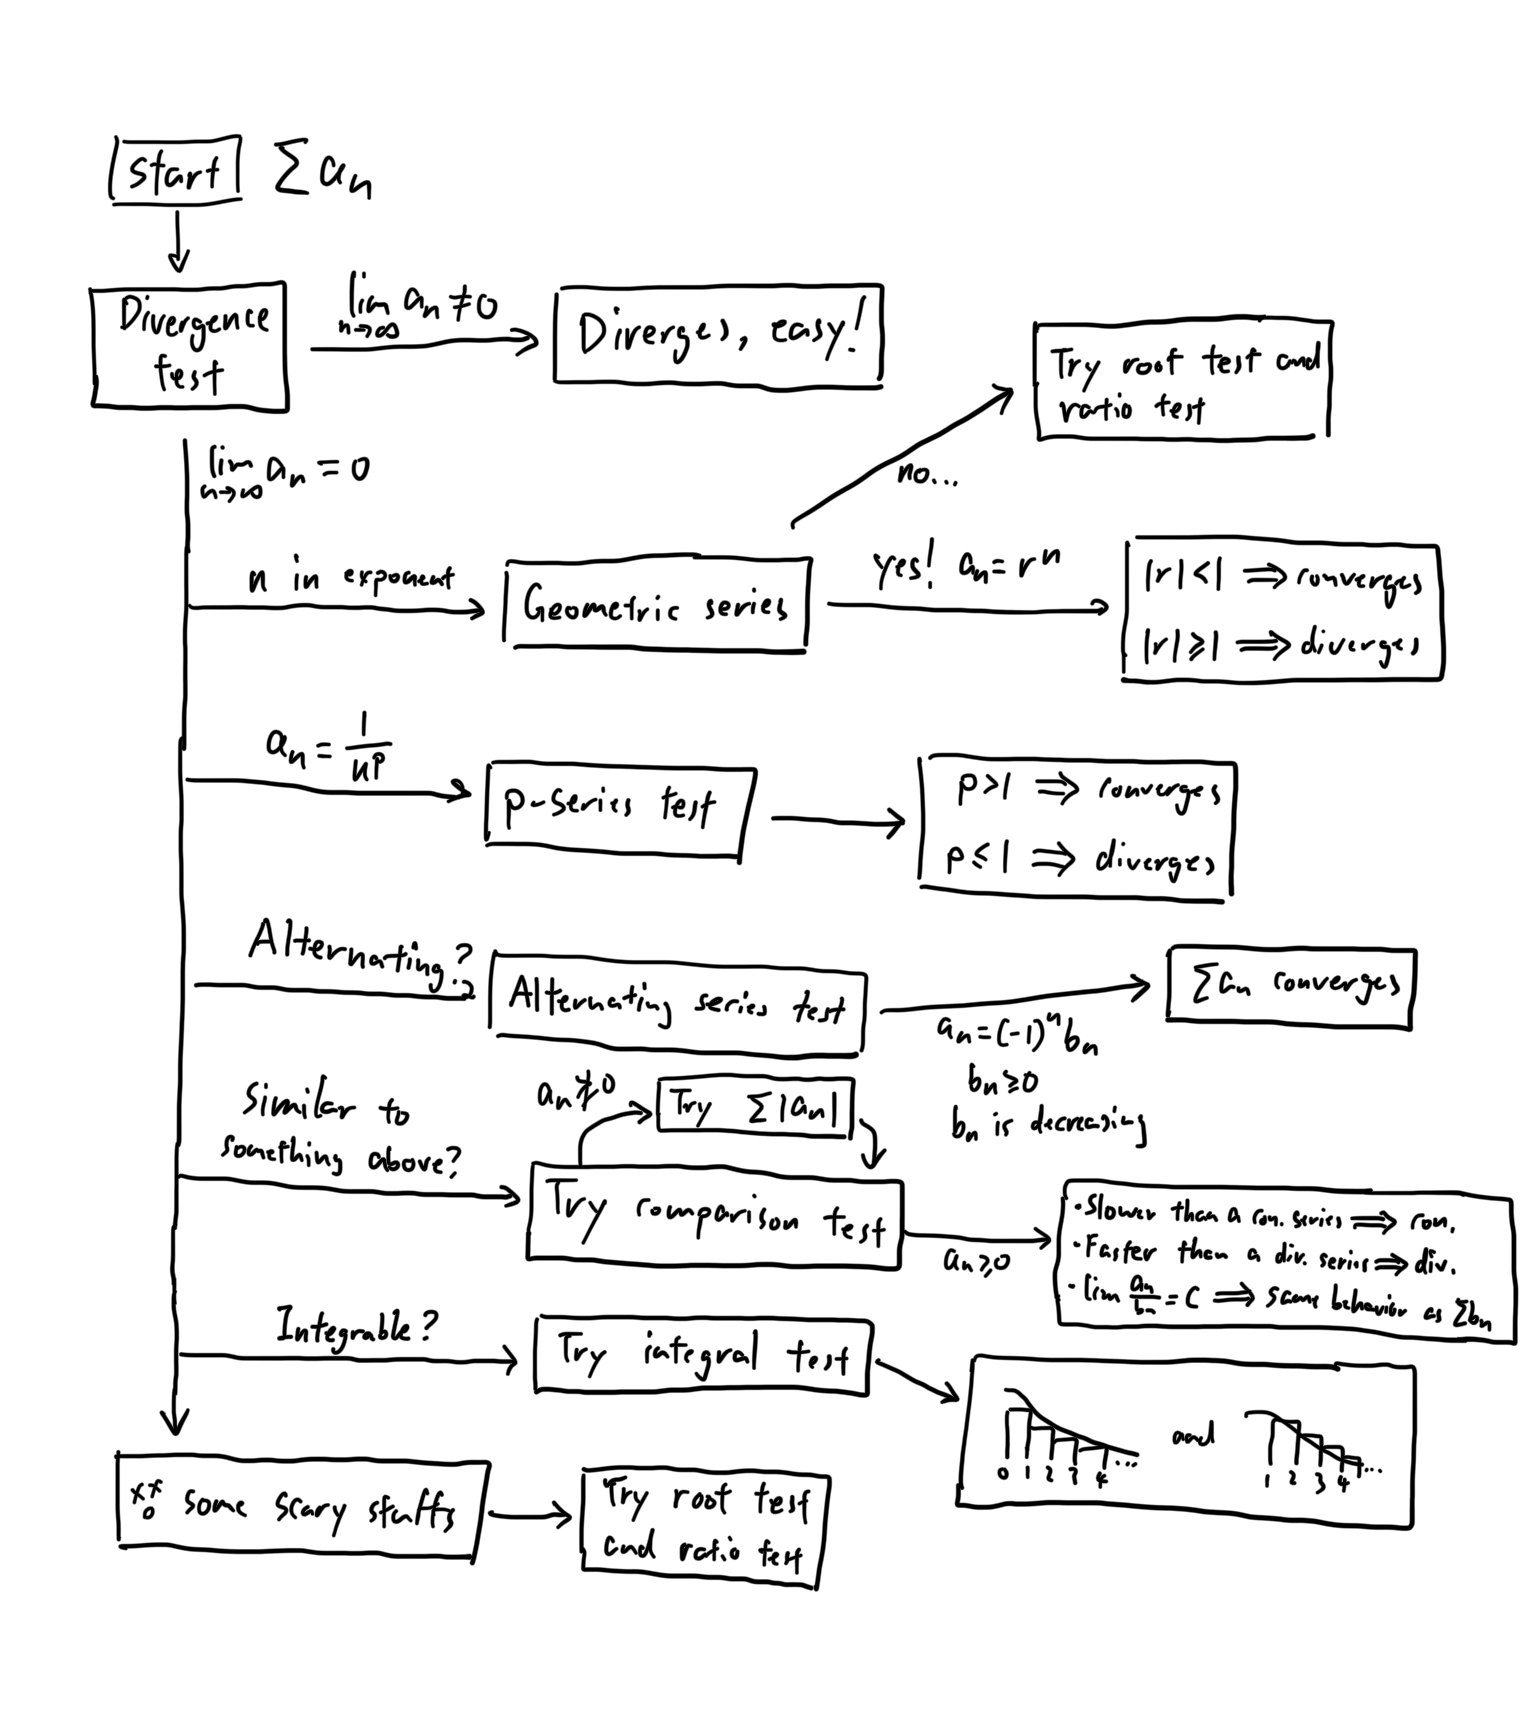
\includegraphics[width=\textwidth]{IMG_0744.PNG}
    \newline
    \small Diagram credit to Raymond Chou who TA-ed MAT 21C in Fall 2020.
    \newline
    \small Don't forget telescoping series! But it is more of a technique for evaluating series than a convergence test.
\end{center}

\end{document}